%----------------------------------------------------------------------------
\chapter{\bevezetes}
%----------------------------------------------------------------------------
% A bevezető tartalmazza a diplomaterv-kiírás elemzését, történelmi előzményeit, a feladat indokoltságát (a motiváció leírását), az eddigi megoldásokat, és ennek tükrében a hallgató megoldásának összefoglalását.
% A bevezető szokás szerint a diplomaterv felépítésével záródik, azaz annak rövid leírásával, hogy melyik fejezet mivel foglalkozik.

In most conventional, "non-smart" houses or flats, utility and convenience devices (eg. lighting, heating, ventilation) are mostly controlled manually by hand via simple switches, knobs or the combination of the two, which requires people to be physically present at the scene to actuate them. In a home equipped with a smart home system, an extra computer and relay or transistor based system is added to them, which assists their actuation from centralized user interface (most often controlled on a smartphone application). Smart home systems can also be extended with digital sensors and other more fine tunable, convenience and security devices (in general just called as "smart" devices), such as temperature and humidity sensors, RGB lights, keycard readers, cameras. The sensors, along with other kinds of input (eg. time of the day, phone sensing) can be used to automate processes, which in turn would require manual interaction, such as turning on or off lights in rooms based on presence, rolling a shutter on or off at a certain time of a day. The general term for this process is called home automation, but this term also means the process of installation and usage a smart home system, so their meaning is almost identical in most contexts.

I believe that a demonstrational "box" model is an adequate and cost-effective solution to try out the usage of smart home systems and to simulate a proper system installed in a real house. During its implementation phase, I tried to follow two basic principles: cost-effectiveness (cheap price for a thesis project) and the usage of open-source software. We can often hear these days, that companies end supporting and updating their not so old, still completely functional products, which make them vulnerable to attacks and contributes to them becoming hazardous waste (take Amazon Echo Look as an example \cite{VergeAmazonEchoLook}). This problem can be mitigated to some extent with the usage of actively maintained open source software available to such devices, because this way they can run up-to-date software years after manufacturing, furthermore the devices chosen for the thesis project can be later repurposed in other projects.

The demand for smart home system and home automation technology has been steadily increasing since their inception and there is active market potential in them (the Worldwide Economic Forum predicts it could react 13 trillion dollars by 2030). Initially, they were considered only as a convenience product (with remote control, a centralized control interface), but since then they have also become a solution of efficiency and safety. Examples for the earlier are automatized heating and motion controlled lights, for the latter are recorded security footage and its analysis, support of handicapped people. \cite{ChakSHS}
% todo source

% todo sw is just as much important as hw?
% todo connection to iot

\section{Motivation, previous work}

My motivation behind choosing this thesis project was mostly my previous work on the topic and also that it combines more fields of expertise: various fields in Information Technology along with basic electronics.

For Training Project Laboratory, me and my two fellow students used an ESP-based microcontroller to control a few small electric components connected to it, which in large resembled a house's utilities. However, this was only a very rudimentary breadboard model, with continuous debug printing to the serial console and only a potentiometer and two buttons as inputs, but it was useful to familiarize ourselves with the usage and programming of a modern microcontroller liked by many hobby enthusiasts.

Throughout Project Laboratory, I took the project further and made a proper shoebox smart home system model. Along with a basic floorplan for various rooms and electronic components placed in them, it featured a web-controllable user interface. Its software architecture was comprised of three main components: a JavaScript backend responsible for maintaining the components' status and communication between the microcontroller and user, microcontroller code for controlling the electronic components (reading sensor data, setting output for actuators), receiving and sending data to the backend and finally a React-based frontend to send commands and receive readings to and from the backend.
%I decided to apply with it for Gadget Competition 2024 (organized by BME-MIT) and achieved 4th place on the competition.
% todo maybe pic of box and ui
For the Thesis Project, I've decided to continue work with the shoebox model, but focus more on the software side of improvement - the hardware, electronic components inside the box have remained mostly the same. I believe that the software of my Project Laboratory project was sufficient for showcasing simple smart home use cases in a demo environment, however would have been harder to further develop to extend with more devices and features than using already existing open-source smart home software with good community support, which I had also been looking forward to try out.

\section{A brief history of smart home systems, protocols}
% - development of protocols (not only used for smart homes) wifi, iot, zigbee, z-wave
% - cloud, subscription world and future, why local hosting is important

The Third Industrial Revolution's main innovation was the usage of IT and computer technology in order automate certain industrial processes and achieve a substantial speed up of tasks previously done via manual labor. \cite{UpkeepIndRev}
The appearance of Programmable Logic Controllers (PLCs) and innovation in Robotics made it easier, than ever to precisely control electric devices with a certain logic in industrial installations with much less human supervision. This aspect of computer-based electric and electronic device control is also important for the functioning of smart home systems, however the latter only started to be developed much more later, after a demand appeared for them and manufacturers started to experiment. %todo source

\subsection{Protocols}

The first major breakthrough, that helped the conception of the home automation field was the introduction of the X10 protocol and the devices utilizing it in the 1970s. X10 made it possible to control one lamp and one appliance via a remote control and a central control console by utilizing the house's already existing electrical wiring (on the same phase) to send commands from the control device the the appliances. Later versions of X10-based systems made it possible to control even more devices with more customization option and the platform still has some popularity among home automation enthusiasts, although it's mainly criticized for its lack of encryption. \cite{CavaX10}

However it took a while, before more sophisticated home automation solutions appeared, that utilized computers for controlling the apparatus and interfacing the users. One important aspect of such systems is the way devices communicate to each other, which also required a lot of research and development.
After the introduction of wired computer networking protocols, suchs as Ethernet, TCP/IP, which became the basis for the World Wide Web (WWW) in the early 90s, wireless computer networking, building and home automation related communication protocols and devices also appeared, but only later in the late 90s.
Although many automation devices could be networked via a UTP cable and utilize the aforementioned Ethernet and TCP/IP protocols, the development and usage of wireless protocols made their installation easier and contributed to their spread due to the lower cost of not having to run network cables all around the house besides the power cables and the possibility to make devices portable. IoT, or Internet of Devices is a collective term for the network of physical devices, vehicles, home appliances, and other embedded devices which connect to each other and exchange data. \cite{ShafiqIoTAttacks} Home automation devices make heavy use of IoT as well, besides other systems, such as smart grids, autonomous vehicles.

The first version of Wi-Fi was introduced in 1997 and made it possible for devices to comminicate wirelessly with a relatively high bandwidth of 2 Mbps on the 2.4Ghz ISM band, mainly designed as a Local Area Network (LAN) and Internet access protocol for home and office usage on laptops, PDAs and other mobile computers. Later versions improved bandwidth and some versions utilize the 5 and 6 GHz ISM bands instead for higher bandwidth - but at a lower range. \cite{IEEEWiFi}

Z-Wave, introduced in 1999 is a wireless communication protocol designed for residential and commercial building automation and utilizes the 900 MHz range for transmission, therefore achieves higher range at a lower bandwidth, still sufficient for the targeted kinds of devices, such as garage openers, smoke alarms and motions sensors. \cite{PCMagZWave}

Zigbee, an other low-power communication protocol was introduced in 2003 and originally used the 2.4 GHz ISM band (the 2023 Pro specification added 800-900 MHz support). It is mainly used in home automation, medical data collection, and industrial control systems. \cite{DigiZigbee}

Bluetooth is a short-range wireless protocol introduced in 1997, mainly used to wirelessly connect peripherals to mobile phones, desktops, and laptops and point-to-point mobile phone connection. \cite{IntelBluetooth} Some of the most common Bluetooth accessories include mice, keyboards, speakers, and headphones. It is less used in home automation, however can be useful in some situations, including detecting one's presence with their phone's transmitted Bluetooth signal. %todo maybe write more about BT, BTLE

Although wireless communication can be useful for many home automation related use cases, it might not always be the best solution opposed to a wired connection. A solution to ease the burden of wiring is Power over Ethernet (PoE), which was introduced in 2003. \cite{TTPoE} Power over Ethernet is a technology in wired Ethernet local area networks that enables the transmission of power necessary for every operating device to be carried on the same Ethernet cable, that is used for data transmission, therefore eliminates the need of a separate power cord running to the device. Devices, that make active use of it include VoIP phones, video surveillance cameras and high power LED lights. It requires the recipient device to have the necessary power converter electronics, that converts the higher voltage to the required device voltage and the source to be able to power it. If the source device (most likely a switch) it is connected to isn't PoE capable, it can still made so with the usage of a PoE adapter. For PoE, almost always a higher voltage is used than the recipient's internal, because the higher voltage has less resistance at the same amount of power transmitted.

Smart home products really became popular in the 2010s, however with this came a problem among the many products by many manufacturers: they mostly used their own ecosystem, on top of certain standard protocols and this made their cooperation hard, users had to use different interfaces and ecosystems for each owned device. A proposed solution to allow products from different manufacturers to securely communicate in a standardized manner is Matter. \cite{PCMagMatter} The working group behind it was formed in 2019 by Amazon, Apple, Google and other big corporations, and it's being actively developed and adapted by many manufacturers for more and more types of appliances. It is based on the Internet Protocol and uses other existing protocols for the underlying connections, such as Wi-Fi and Bluetooth.
% todo http, rest api, json, websocket insert json code as figure
% maybe thread, mqtt

\subsection{Solutions}

In the mid 2000s, companies with a strong focus on home automation products started appearing, such as Control4 in 2004, Insteon and Savant in 2005. \cite{Control4about} \cite{WPInsteonFirstLook} \cite{SavantCompInfo}\break
Later in the early 2010s, many big IT corporations also jumped onto the hype around smart home systems and released products on the market, often bundled with their voice assistant solutions. This was also helped by the spread of smartphones after the introduction of early iPhone and Android phones and tablets at the end of the earlier decade. Manufacturers could use their software platform to build applications for interfacing users and it also meant that they could make their systems cheaper by only optionally including a control console device as that could be substituted by the phones or tablets. Such platforms include Amazon's Alexa Smart Home with their Alexa voice assistant and Echo smart speakers, Google's Home with their Nest devices and Assistant voice assistant, Apple's HomeKit software platform. \cite{AmazonAlexaSH} \cite{GoogleHome} \cite{GoogleAssistant} \cite{AppleHome} Since then, many home automation, smart home devices and solutions have appeared on the market, the industry has great market potential with a plentiful of competition. \cite{ChakSHS}

A typical smart home system usually includes smart devices, that mostly provide or control home utilities, along with detectors, sensors and other devices facilitating extra services (eg. voice assistant), along with a control utility in the form of a dedicated device or a local or remote computer running a specific control software. Many smart utility devices replace their conventional equivalent (which aren't "smart"), their retrofitting isn't hard. Such utility devices comprise of controllable monochrome or RGB LED lightbulbs and light strips, thermostats for control of heating and cooling (A/C), garage openers, presence detectors, air, humidity and particulate sensors and many more. \cite{TechTargetSH}

In the 2010s, cloud computing technology also started started to get traction, as big IT corporations launched theirs, take Amazon Web Services (AWS), Google Cloud Platform (GCP) and Microsoft Azure as examples. Cloud computing means that such providers provide on-demand delivery of IT resources over the Internet, so that that companies can use this to outsource different portions of their infrastructure instead of having to operate everything themselves. \cite{AWScloud} It can lead to significant cost savings besides the more agile and faster deployments, scaling of resources according to demand. This technology was also beneficial for smart home solutions, for a number of reasons. \cite{ChakSHS} Most modern smart home devices require some form of background IT infrastructure (eg. control server) for management, remote access and data collection, which is something that most customers aren't tech savvy enough to set up themselves and operate, regularly update. The amount of data generated also varies device-by-device, typically security cameras would require the most amount of data to be stored somewhere. Because of the many advantages of cloud technologies, manufacturers started to use cloud technologies extensively for their products and focus less on locally hosted solutions.

However, the usage of cloud technology is a double edged sword for a number of reasons. As for concerns against cloud solutions, the first is being vulnerable to the hosting providers and the reliability of their technologies. Although many big IT companies invest heavily in their technologies, downtimes sometimes occur, during which the usage of a smart home system dependant on it might be limited or not possible. An other big concern is privacy and security: devices reside in people's private lives, therefore should be well-protected against access by external parties. A disgruntled hosting or manufacturer employee, state agency or hackers utilizing a vulnerability or weak passwords might be able gain access to the system and peek into its data, as if the owner's were in Big Brother. \cite{QACloudDisadvantages} % maybe limited control, fb lockout 2021, vendor lock-in

Despite the widespread use of cloud-based solutions, many tech-savvy users decide to only use locally hosted smart home platforms with devices either officially or unofficially supporting this way of operation due to the corcerns associated with cloud-based solutions. This way, users have full control of their smart home infrastructure and data, which when set up for remote access, will be as secure as it's encryption capabilities and scarcity of vulnerabilities. Such users almost always run open-source smart home software platforms. They also prefer to use hardware made out of open-source platforms, microcontrollers (eg. Arduino, ESP) and basic electronics, or use commercial products with aftermarket open-source firmware flashed onto them instead of utilizing the original software from the manufacturer, which uses remote or cloud services. Home Assistant and OpenHAB are good examples for open-source smart home platforms that can be hosted on a local server and have support for smart many devices from different brands and have good community support from their maintainers and users. \cite{HAHomepage} \cite{openHABHomepage} ESPHome and MySensors are two open-source software projects that allow microcontrollers to be easily able to set up in different smart home platforms and control specified electric and electronic devices connected to their pins, eliminating the need to write custom microcontroller code for different platforms, connected components and communication to the control server. \cite{ESPHomeHomepage} \cite{MySensorsHomepage}

\section{Architecture and devices of a typical smart home system}

Every smart home system solution and product is different, however there are a few key concepts and parts, that most solutions follow and share. In this thesis, a typical IoT-based smart home system's architecture and devices are presented with some variations, along with the general concepts that they follow. There are also smart home systems which utilize Artificial Intelligence (AI) and its forms in Machine Learning (ML), Deep Learning (DL) and Neutral Networks (NN), furthermore Multiagent System (MAS) and Image Processing (IP) based smart home systems, however these aren't going to be covered in the thesis due to them being not used in the accomplished physical demo model presented in the upcoming chapters. \cite{ChakSHS}

\begin{figure}[!ht]
    \centering
    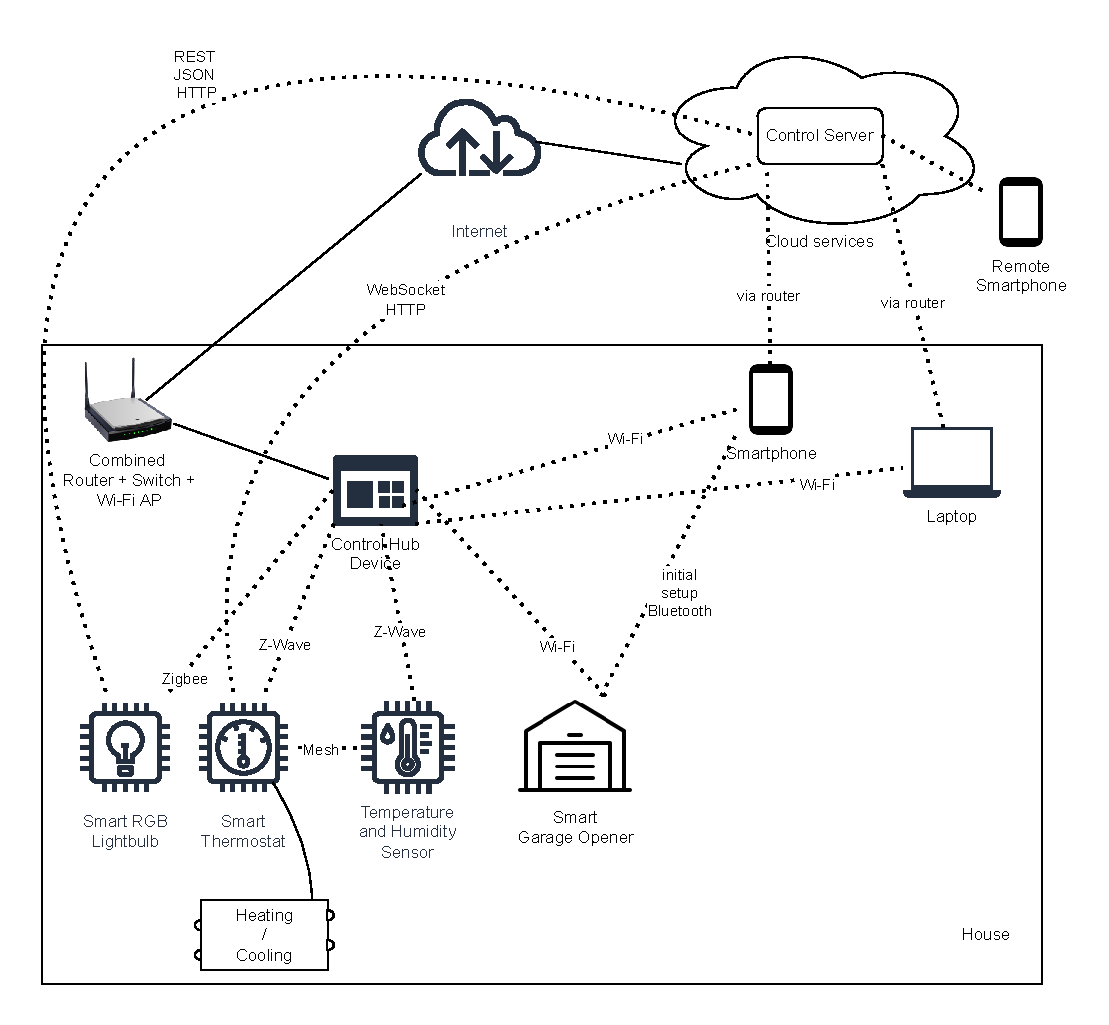
\includegraphics[page=1,keepaspectratio,width=150mm]{figures/sh_architecture_cloud.drawio.pdf}
    \caption{Architecture of a typical cloud-based smart home system}
    \label{fig:SHCloud}
\end{figure}

\begin{figure}[!ht]
    \centering
    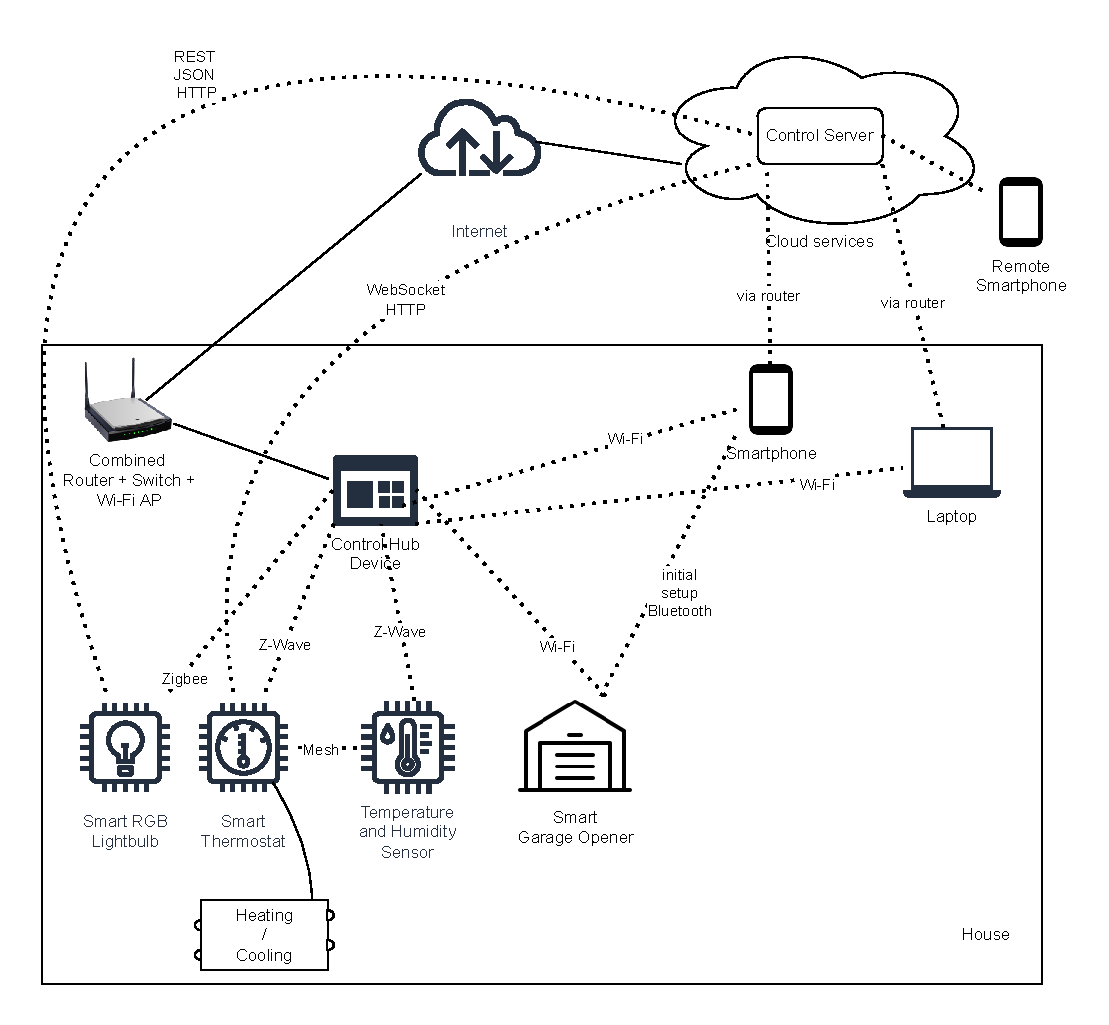
\includegraphics[page=1,keepaspectratio,width=150mm]{figures/sh_architecture_cloud.drawio.pdf}
    \caption{Architecture of a typical locally hosted smart home system}
    \label{fig:SHLocal}
\end{figure}

% todo draw.io diagram of a shs: cloud, locally hosted non-mesh, mesh

Many IoT-based smart home systems use a controller as a brains of operations, although its form of implementation can vary to a great extent according to the specific platform. One form of implementation is a controller "box" or "hub", where a physical device is present, which manages the appliances, collects data and stores it for later review and provides an interface (on the devices itself, or from a smartphone or computer application) for user control. An other controller solution is a specific control software run on a local or remote (many times cloud-based) computer, to which apparatus connect via an IP-based wired or wireless network solution. A control hub device is sometimes combined with remote or cloud services, therefore it can be used as a user interface, while data gets stored at a remote location.

The networking solution between devices are also varied, but they mostly use the aforementioned wired and wireless protocols. Most households have a combined network device that has multiple functionalities, which in some cases are set up as separate dedicated devices. An IP router in a home network is a device that allows communication to the Internet via the Internet Service Provider's (ISP's) modem. An Ethernet Switch is a network device that allows wired Ethernet devices to be connected together to a common medium while also making sure non-broadcast frames are only sent to the destination. A Wi-Fi Access Point is a device that lets Wi-Fi enabled devices, such as smart apparatus besides smartphones and laptops to connect to it's Ethernet network. An aforementioned combined network device has these three functionalities integrated into it, along with others, eg. DHCP server, firewall, Network Address Translation (NAT, for IPv4) and more. Many ISPs also provide such device with an integrated modem, therefore only one device is needed to be deployed to homes and owners needn't purchase a separate besides the modem for the benefit of both parties. Smart devices utilizing cloud or remote servers would address these servers and use the specified default gateway in the network to access them through the Internet, which is shown on \refstruc{fig:SHCloud}. They can also frequently set up from a smartphone, therefore use a Wi-Fi or Bluetooth connection for the initial setup. Some devices with specific wireless protocols, such as Z-Wave and Zigbee can also work in a mesh, in other words, devices can connect to each other directly and forward messages to each other via intermediate nodes, therefore can reach further as if they only communicated to a central node. On \refstruc{fig:SHLocal}, a locally hosted environment is shown, in which devices mostly communicate to the control server and optionally with each other in case of a mesh network and the control server is usually set up to be remote controllable from outside the reach of the home via a firewall rule and NAT.

Smart devices 
- devices:
what processes function in it to make txrx on nw to control of a high power transistor or relay, so the electronics to control the electric parts
sensors
actuators
light



- user interface
backend, api
http, rest, api, json, websocket
controlled from central console
smartphone, tablet app
web interface
% - alexa, google voice, etc voice assistants
% figure to show example


- etc, tadada
